\documentclass[12pt]{article}
\usepackage[utf8]{inputenc}
\usepackage{graphicx} % Allows you to insert figures
\usepackage{amsmath} % Allows you to do equations
\usepackage{import}
\usepackage{enumitem} % for list items
\usepackage{tikz}
\usetikzlibrary{calc, shapes.geometric}
\usepackage[latte,styleAll]{catppuccinpalette}
\usepackage{float} % for \begin{figure}[H]
\usepackage{caption}
\usepackage[english]{babel}
\usepackage{csquotes, lipsum, ragged2e}
\usepackage[dvipsnames]{xcolor}
\usepackage[backend=bibtex, language=auto, autolang=other, bibencoding=utf8]{biblatex}
\usepackage{fontspec}
\usepackage{media9}
\usepackage{geometry} % Formats the paper size, orientation, and margins
\geometry{
 a4paper,
%  total={8.5in,11in},
 left=20mm,
 top=20mm,
 }

\setlength{\parskip}{1em} % paragraphs separated by one line
\usepackage[format=plain,
            font=it]{caption} % Italicizes figure captions
\setsansfont{P052}[
    Path=./fonts/palladio/,
    Scale=0.85,
    Extension = .ttf,
    UprightFont=*-Roman,
    BoldFont=*-Bold,
    ItalicFont=*-Italic,
    BoldItalicFont=*-BoldItalic
]
\setmonofont{IBMPlexMono}[
    Path=./fonts/IBMPlex/,
    Scale=0.85,
    Extension = .ttf,
    UprightFont=*-Regular,
    BoldFont=*-Bold,
    ItalicFont=*-Italic,
    BoldItalicFont=*-BoldItalic
    ]
\newfontfamily\virgil{Virgil}[
    Path=./fonts/,
    Extension=.ttf % Change to .otf if applicable
]
% SET GLOBAL DEFAULT FAMILY
\renewcommand{\familydefault}{\sfdefault}
% SET GLOBAL DEFAULT FAMILY
% \usepackage[T1]{fontenc}
% \usepackage{tgbonum}
% https://www.overleaf.com/learn/latex/Font_typefaces
\definecolor{kwcolor}{rgb}{0.902,0.75,0.478}
\definecolor{sblue}{HTML}{C1E8F7}
\definecolor{syellow}{HTML}{F1F4C1}
\definecolor{sorange}{HTML}{FFE2BB}
\definecolor{sstart}{HTML}{FBE0E0}
\definecolor{sgreen}{HTML}{CCE7CF}
\definecolor{spurple}{HTML}{C5BEDE}

\usepackage{xcolor}
\definecolor{BasePythonColor}{HTML}{C678DC}
\usepackage{listings}
\lstdefinestyle{python}{
  backgroundcolor=\color[rgb]{0.91,0.925,0.929},
  language={python},
  breaklines=true,
  showstringspaces=false,
  breakatwhitespace=true,
  stringstyle = {\color{CtpGreen}},
  commentstyle={\color{CtpOverlay1}},
  basicstyle = {\small\color{CtpText}\ttfamily},
  keywordstyle = {\color{CtpMauve}},
  keywordstyle = [2]{\color{CtpBlue}},
  keywordstyle = [3]{\color{CtpBlue}},
  keywordstyle = [4]{\color{CtpLavender}},
  keywordstyle = [5]{\color{CtpPeach}},
  keywordstyle = [6]{\color{CtpTeal}},
  otherkeywords = {<, ||, =, ?},
  morekeywords = [2]{import, if, def, repr},
  morekeywords = [3]{Model, forward, all, format, nn, functional, nn.Module},
  morekeywords = [4]{@page},
  morekeywords = [5]{exception, do_some_for_pages, @page, @admin},
  morekeywords = [6]{<, ||, =, ?},
  framexleftmargin=3pt,
  framextopmargin=1pt,
  framexbottommargin=1pt, 
  frame=tb, framerule=0pt,
}
\lstdefinestyle{C}{
    belowcaptionskip=1\baselineskip,
    breaklines=true,
    numbers=none, 
    basicstyle=\footnotesize\ttfamily,
    keywordstyle=\bfseries\color{green!40!black},
    commentstyle=\itshape\color{purple!40!black},
    identifierstyle=\color{blue},
    backgroundcolor=\color[rgb]{0.91,0.925,0.929},
    framexleftmargin=1pt,
    framextopmargin=1pt,
    framexbottommargin=1pt, 
    frame=tb, framerule=0pt,
    showstringspaces=false
}
\definecolor{xsocial}{HTML}{1C9BEF}
\definecolor{xtitle}{HTML}{1E6A41}
\definecolor{xlink}{HTML}{036EE8}
% Define a custom command
\newcommand{\customtext}[3]{% 
    \vspace{#2} % #2 is the vertical spacing
    \fontsize{13}{8}\textcolor{#1}{\textit{#3}}% #1 is the color, #3 is the text
}
\newcommand{\bandi}[1]{\textbf{\textit{#1}}}
% \newcommand{\sidecite}[1]{\scriptsize\ \textcolor{blue}{$ \mathbf{^{#1}}$}\normalsize}
\newcommand{\sidecite}[1]{\textsuperscript{\textcolor{blue}{\textbf{\scriptsize#1}}}}
\newcommand{\customtitle}[1]{\fontsize{14}{8}\textcolor{xtitle}{\textit{#1}}\\}
\usepackage{hyperref}
\hypersetup{
    colorlinks=true,
    linkcolor=xlink,
    filecolor=xlink,      
    urlcolor=xlink,
    pdftitle={Overleaf Example},
    pdfpagemode=FullScreen,
}

\urlstyle{same}
\usepackage{fontawesome}
\begin{document}
\linespread{1.2}\selectfont
\title{GPGPU Programming with CUDA}
\author{Marvin}
\date{\today}
% \maketitle
% PAGE 1
\begin{figure}[!htb]
    \begin{minipage}[t]{0.65\textwidth}
    {\sffamily 
    \fontsize{21}{8}\textcolor{xtitle}{\textit{Scaling ViTs across Training Compute}}\\
    \fontsize{9}{8}\textcolor{xtitle}{\textit{\ by \href{https://www.linkedin.com/in/marvin-mboya-b7bb81195/}{Marvin\ \faLinkedinSquare}}}\\
    }\\
    [-0.3cm]
    \textcolor{xtitle}{{\it A journey across optimization levels}}\\
    [0.2cm]
    \normalsize
    \raggedright
    Looking back at when we could only reliably produce Shakespearean poetry with {\it RNNs}, a thin line between hallucinations 
    and poetry, one can see why Google open sourcing Transformers was the just needed {\it krabby patty secret formula} to SOTA 
    models toppling leaderboards every coming week, and copyright lawsuits enriching the lawyers in the same way that AI ideas 
    could be well thought out as a well pipelined autocomplete service driving some startups.\\ 
    % Too bad {\it Plankton} lives under the sea!\\
    This article is a no exception, {\it thanks Transformers!}, written from the curiosity that inspires I to 
    sit on the shoulders of giants, intellectually speaking, and start off this chain of optimization across languages and hardware 
    stack that only climaxes limited to the largest GPU compute I can access without feeling like I have leaked my AWS cloud keys 
    to the best crypto miners in the east continents!
    \vspace{1.5em}\\
    \fontsize{14}{8}\textcolor{xtitle}{\textit{Back in time}}\\
    {\it Vaswani et al.} didn't understand the gravity of their research$^1$ when they lightly ended their paper, but 
    it inspired to generalize learning in the natural language domain, being largely parallelizable and solving saturation in 
    training performance for increased training data.\\
    Recurrent Neural Networks$^2$ was the precursor to this, its encoder that generates the latent space representation of the input tokens
    working in such a way that it captures the entire meaning of the input sentence in its final hiddetn state. This processing of the 
    entire input text was its drawback as it could not access intermediate hidden states hence not capturing dependencies within words
    in the sentence.\\
    \vspace{1em}
    \small \textcolor{xtitle}{\textbf{\textit{Sweet sauce of Transformers}}}\\
    \normalsize
    Parallelizability, scaled dot product attention, and scaling of models to unprecedented size while maintaining trainability.
    
    \end{minipage}
    \hspace{25pt}
    \begin{minipage}[t]{.4\textwidth}
      \raggedright
      \scriptsize 
      $^1$ 	\href{https://arxiv.org/abs/1706.03762}{arXiv:1706.03762}\\
      {\it Attention is all you need}\\
      {\it Vaswani et al. 2017}\\
      \vspace{2em}
      $^2$ RNNs can be understood using a special key word, {\it \bf recurrent}, meaning to recur, where each hidden 
      state would have a loop within itself and also includes the compounded outputs of all the previous hidden states,
      hugely based on the concept of a Markov model\\
      \vspace{2em}
      {\bf Markov process} is a stochastic process with the properties:
      \begin{itemize}[left=0pt,topsep=0pt,itemsep=-1ex,parsep=0ex]
        \item number of posssible states is finite
        \item outcome at any state depends only on outcomes pf previous states
        \item probabilities are constant over time 
      \end{itemize}
      where a \textit{\textbf{stochastic process}} can be said as a probability distribution over a space of paths;
      this path often describing the evolution of some {\bf random variable} over time.\\
      \vspace{1em}
      A random variable, despite its name, is never random, and not a variable, it is a deterministic function.\\
      \vspace{1em}
      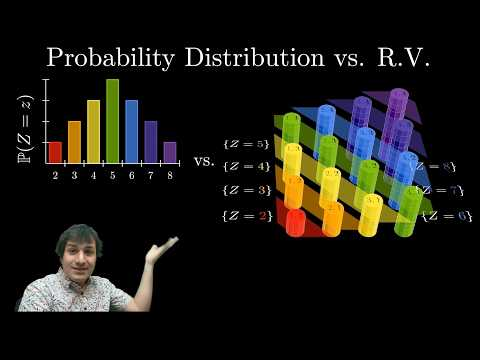
\includegraphics[width=0.5\textwidth]{images/rvnotrandom.jpg}\\
      Thanks to Dr Mihai for this awesome video explaining much on this
      \tiny \url{https://youtu.be/KQHfOZHNZ3k?si=jWPeMLZV0EF76mGz}
    \end{minipage}
\end{figure}
\pagebreak
% PAGE 2
\begin{figure}[!htb]
    \begin{minipage}[t]{0.65\textwidth}
    \raggedright
    \customtext{xtitle}{0em}{From a black box approach}\\
    Given a text {\small \textit{\textbf{The ruler of a kingdom is a}}} with the next likely word 
    being \textit{\textbf{\small king}}, humanly thinking, how is the input sentence then passed to a 
    Transformers model?\\ 
    Basically, computational models cannot process strings, hence it needs conversion to a vector of integers, each word (or subword) 
    uniquely mapped to a corresponding integer, a process known as {\it tokenization}. A basic form 
    would be a hashmap of words to integers and vice versa for getting a word from index of maximum 
    probability in softmaxed one-dimensional distribution of output float values \sidecite{3}.\\
    \vspace{0.5em}
    Implementing a simple tokenizer based on the vocabulary\sidecite{4} we have, 
\begin{lstlisting}[language=python,style=python,,basicstyle=\ttfamily\footnotesize]
text = "The ruler of a kingdom is a"
text = text.lower() # making tokenizer case insensitive 
text = text.split() # getting individual words 
# as separated by spaces 
vocab = list(sorted(set(text)))
words_to_ids = {word:i for i, word in enumerate(vocab)}
ids_to_words = {v:k for k,v in words_to_ids.items()}
\end{lstlisting}
Great, now we have lookup tables (the last two lines), and a naive preprocessing of text needed 
before tokenization.  So then, let's tokenize \textcolor{xtitle}{the kingdom had another ruler}.
Wait?! The lookup table does not have the words \textcolor{xtitle}{"another", "had", "another"}! 
Let's improve it so any word not part of the original vocabulary be assigned a new unique id\sidecite{5}.
\begin{lstlisting}[language=python,style=python,,basicstyle=\ttfamily\footnotesize]
words_to_ids = {word:i for i, word in enumerate(vocab)}
ids_to_words = {v:k for k,v in words_to_ids.items()}
def lookup(word):
    try: 
        id = words_to_ids[word]
    except KeyError:
        vocab.append(word)
        words_to_ids[word] = len(vocab) - 1
        ids_to_words[len(vocab)-1] = word 
        id = words_to_ids[word]
    return id 
\end{lstlisting}
    \end{minipage}%
    \hspace{25pt}
    \begin{minipage}[t]{.4\textwidth}
      \raggedright
      \scriptsize 
      $^3$ the commonly used tokenizer is tiktoken, using a concept called Byte-Pair Encoding to 
      map subwords to ids using a look-up table that takes into account frequencies of subwords.\\
      \vspace{2em}
      $^4$ vocabulary {\tiny $\sim$} set of unique words (or subwords based on the tokenization strategy) 
      in all words of the entire training dataset used to train a particular large language model.\\
      \vspace{2em}
      $^5$ our look-up tables are very much capable of any encoding and decoding (for the tiny tiny vocabulary).
    \end{minipage}
\end{figure}
% PAGE 3
\pagebreak
\begin{figure}[!htb]
    \begin{minipage}[t]{0.65\textwidth}
    \raggedright
    \customtext{xtitle}{0em}{Trying our shiny code}\\
\begin{lstlisting}[language=python,style=python,,basicstyle=\ttfamily\footnotesize]
sentence = "the kingdom had another ruler"
tokens = [lookup(word) for word in sentence.lower().split()]
print(tokens)
# [5, 2, 6, 7, 4]
words_gotten = [ids_to_words[id] for id in tokens]
sentence_gotten = " ".join(words_gotten)
print(sentence_gotten)
# "the kingdom had another ruler"
\end{lstlisting}
\textbf{\textit{\small Note}} that the above implementation of tokenization is to help you understand a baseline of what happens 
under the hood in conversion of what models cannot deal with, strings, to a format that can be computationally 
crunched.\\
Hoever, when looking into the Transformers model architecture as outlined in the paper\sidecite{1}, also in\sidecite{6}
for convenience, it is seen that the first block is an Embedding block.\\
\customtext{xtitle}{1em}{What about the Embeddings block?}\\
Well, the vector of integers as input in itself cannot capture rich latent representations of the input tokens, 
so the Embeddings block\sidecite{7} does just that, mapping the tokens to higher dimensions. The embeddings block is usually 
\bandi{V} by \bandi{D}, where \bandi{V} is the size of the vocabulary, and \bandi{D} is an abstract dimension of your choosing, 
the higher the better, but more computationally expensive and longer to process.\\
Using PyTorch, an Embeddings block of {\it D being 3} can be implemented as:
\begin{lstlisting}[language=python,style=python,,basicstyle=\ttfamily\footnotesize]
import torch, torch.nn as nn 
V, D = len(vocab), 3
emb = nn.Embedding(V,D)
higher_emb_tokens = emb(torch.tensor(tokens))
print(higher_emb_tokens.shape) # torch.Size([5, 3])
\end{lstlisting}
One of the best LLMs ever open sourced by Meta, the Llama 3, the 3 billion parameter size variant, has its vocabulary with {\it 128K} tokens.
and the embedding dimensions, \bandi{D}, being 3072.
    \end{minipage}%
    \hspace{25pt}
    \begin{minipage}[t]{.4\textwidth}
      \raggedright
      \scriptsize 
      $^6$ Transformers architecture\\
      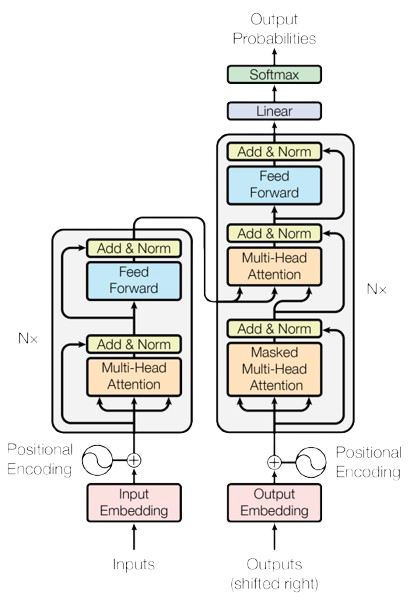
\includegraphics[width=\textwidth]{images/transformers.png}\\
      \vspace{2em}
      $^7$ {\it nn.Embedding} is just {\it nn.Linear} but only that {\it nn.Embedding} simplifies retrieving rows from its weights 
      such that you don't pass it one hot vectors but just indeces basically same as the position of the single {\it 1s} in the 
      one-hot vector you would have passed to {\it nn.Linear}
    \end{minipage}
\end{figure}
\pagebreak
% PAGE 4
\begin{figure}[!htb]
    \begin{minipage}[t]{0.65\textwidth}
    \raggedright
    \customtext{xtitle}{0em}{Positional Encoding}\\
    Before the Multi-Head Attention (MHA) block, the positional encoding is attached to the graph to constitute the position information and 
    this allows the model to easily attend to relative positions.
    Why is that? Well, the MHA block is permutation-equivariant, and cannot distinguish whether an input comes before another one in the 
    sequence or not.\\
    The meaning of a sentence can change if words are reordered, so this technique retains information about the order of the words in a sequence.\\
    Positional encoding is the scheme through which the knowledge of the order of objects in a sequence is maintained.\\
    This post by Christopher\sidecite{8} highlights the evolution of positional encoding in transformer models, a worthy read! For this article, 
    let's focus on the rotary positional embedding (RoPE){\scriptsize\ \textcolor{blue}{$\mathbf{^9}$}}.\\    
    % \vspace{0.5em}
    % \customtext{xtitle}{1em}{Why this encoding?}\\
    % Previous approaches to encoding did first incorporate positional information to the context representations before transforming them to queries, keys and values. 
    % Why is this not good? Well, for linear self-attention architecture, this bias disrupts low-rank factorization hence forcing 
    % explicit computation of the position bias matrix.
    Let's making a few things clear, 
    \begin{itemize}[left=0pt,topsep=0pt,itemsep=-1ex,parsep=0ex]
        \item previous position encodings were done before the MHA block, this is done within it.
        \item RoPE are only applied to the queries and the keys, not the values. 
        \item RoPE are only applied after the vectors $\vec{q}$ and $\vec{k}$ have been multiplied by the 
        \bandi{W} matrix in the attention mechanism, while in the vanilla transformer they're applied before.
      \end{itemize}
    \vspace{1em}
    The general form of the proposed approach for RoPE is as in page 5 for a sparse matrix with pre-defined 
    parameters $\Theta=\{\theta_i=10000^{-2(i-1)/d}, i\in[1,2,...,d/2]\}$\\
    which can be implemented in code as 
\begin{lstlisting}[language=python,style=python,,basicstyle=\ttfamily\footnotesize]
assert d % 2 == 0, "dim must be divisible by 2"
i_s = torch.arange(0,d,2).float()
theta_s = 10000 ** (- i_s / d).to(device)
\end{lstlisting}
where {\it device} is code that chooses the compute device.
\begin{lstlisting}[language=python,style=python,,basicstyle=\ttfamily\footnotesize]
device = torch.device(
    "cuda" if torch.cuda.is_available() else (
    "mps" if torch.backends.mps.is_available() else "cpu"
    )
)    
\end{lstlisting}
   \end{minipage}%
    \hspace{25pt}
    \begin{minipage}[t]{.4\textwidth}
      \raggedright
      \scriptsize 
      $^8$ \tiny{\url{https://huggingface.co/blog/designing-positional-encoding}}\\
      \scriptsize 
      { \it You could have designed state of the art positional encoding}\\
      {\it Christopher Fleetwood}\\
      \vspace{2em}
      $^9$ 	\href{https://arxiv.org/pdf/2104.09864}{arXiv:2104.09864}\\
      {\it RoFormer: Enhanced Transformer with Rotary Position Embedding}\\
      {\it Su et al. 2022}\\
      \vspace{2em}
    \end{minipage}
\end{figure}
% PAGE 5
\pagebreak
\begin{figure}[!htb]
    \begin{minipage}[t]{0.65\textwidth}
    \raggedright
    Given the computational efficient realization which is what we're aiming at getting 
    \begin{equation*}
        \resizebox{.75\hsize}{!}{$
        \boldsymbol{R}_{\Theta,m}^d\boldsymbol{x}=
        \begin{pmatrix}
            x_1\\
            x_2\\
            x_3\\
            x_4\\
            \vdots\\
            x_{d-1}\\
            x_d
        \end{pmatrix} 
        \otimes
        \begin{pmatrix}
            \cos m\theta_1\\
            \cos m\theta_1\\
            \cos m\theta_2\\
            \cos m\theta_2\\
            \vdots\\
            \cos m\theta_{d/2}\\
            \cos m\theta_{d/2}\\
        \end{pmatrix}
        +
        \begin{pmatrix}
            -x_2\\
            x_1\\
            -x_4\\
            x_3\\
            \vdots\\
            -x_d\\
            x_{d-1}
        \end{pmatrix} 
        \otimes
        \begin{pmatrix}
            \sin m\theta_1\\
            \sin m\theta_1\\
            \sin m\theta_2\\
            \sin m\theta_2\\
            \vdots\\
            \sin m\theta_{d/2}\\
            \sin m\theta_{d/2}\\
        \end{pmatrix}
        $}
    \end{equation*}
    Having implemented $\vec{\theta}$, next let's implement {\it $m\vec{\theta}$} by way 
    of an outer product\sidecite{10}\\
\begin{lstlisting}[language=python,style=python,,basicstyle=\ttfamily\footnotesize]
m = torch.arange(context_len, device=device)
freqs = torch.outer(m, theta_s).float()    
\end{lstlisting}
\begin{equation*}
    \resizebox{.8\hsize}{!}{$
    m\vec{\theta}={\text{freqs}}=
    \begin{pmatrix}
      m_1\theta_1, m_1\theta_2, \ldots, m_1\theta_{d/2-1}, m_1\theta_{d/2}\\
      m_2\theta_1, m_2\theta_2, \ldots, m_2\theta_{d/2-1}, m_2\theta_{d/2}\\
      \vdots\hspace{2.5em}\vdots\hspace{2em}\ldots\hspace{2em}\vdots\hspace{2.5em}\vdots\\
      m_{\text{ctx\_len}}\theta_1, m_{\text{ctx\_len}-1}\theta_2,\ldots, m_{\text{ctx\_len}-1}\theta_{d/2-1}, m_{\text{ctx\_len}-1}\theta_{d/2}\\
    \end{pmatrix}
    $}
\end{equation*}
It is then needed to get the complex numbers for the resulting matrix of size context len by $d/2$.
\begin{lstlisting}[language=python,style=python,,basicstyle=\ttfamily\footnotesize]
freqs_complex = torch.polar(torch.ones_like(freqs),freqs)
\end{lstlisting}
which then gives the polar form of each element in the matrix, such that 
\begin{equation*}
    \resizebox{1.1\hsize}{!}{$
    e^{im\vec{\theta}}=
    \begin{pmatrix}
        \cos(m_1\theta_1)+i\sin(m_1\theta_1), \cos(m_1\theta_2)+i\sin(m_1\theta_2),\ldots,\cos(m_1\theta_{d/2})+i\sin(m_1\theta_{d/2})\\
        \cos(m_2\theta_1)+i\sin(m_2\theta_1), \cos(m_2\theta_2)+i\sin(m_2\theta_2),\ldots,\cos(m_2\theta_{d/2})+i\sin(m_2\theta_{d/2})\\
        \vdots\hspace{8em}\vdots\hspace{8em}\ldots\hspace{8em}\vdots\hspace{8em}\vdots\\
        \cos(m_{cl}\theta_1)+i\sin(m_{cl}\theta_1), \cos(m_{cl}\theta_2)+i\sin(m_{cl}\theta_2),\ldots,\cos(m_{cl}\theta_{d/2})+i\sin(m_{cl}\theta_{d/2})\\
    \end{pmatrix}
    $}
\end{equation*}
Let's consider a subset of the inputs and a subset of the matrix above, then\\
\vspace{-2.5em}
\begin{equation*}
    \resizebox{0.95\hsize}{!}{$
    \begin{aligned}
    \vec{x}=& \begin{pmatrix}
        x_1\\x_2\\x_3\\x_4
    \end{pmatrix}
    = \begin{pmatrix}
        (x_1\hspace{2em}x_2)\\(x_3\hspace{2em}x_4)
    \end{pmatrix}
    = \begin{pmatrix}
        x_1+ix_2\\x_3+ix_4
    \end{pmatrix}
    \otimes
    \begin{pmatrix}
        f_{11} + i\hat{f}_{11}\\
        f_{12} + i\hat{f}_{12}
    \end{pmatrix}
    \text{,\ where} 
    \begin{cases}
        f_{11} = \cos(m_1\theta_1)\\
        \hat{f}_{11}=\sin(m_1\theta_1)\\
        f_{12} = \cos(m_1\theta_2)\\
        \hat{f}_{12}=\sin(m_1\theta_2)\\
    \end{cases}\\
    =\ & (x_1 + ix_2)(f_{11} + i\hat{f}_{11})\ =\ x_1f_{11}-x_2\hat{f}_{11}+i(x_1\hat{f}_{11}+x_2f_{11})\\
    & \text{meaning} 
    \begin{pmatrix}
        x_1+ix_2\\x_3+ix_4
    \end{pmatrix}
    \otimes
    \begin{pmatrix}
        f_{11} + i\hat{f}_{11}\\
        f_{12} + i\hat{f}_{12}
    \end{pmatrix}\\
    = &
    \begin{pmatrix}
        x_1f_{11}-x_2\hat{f}_{11}+i(x_1\hat{f}_{11}+x_2f_{11})\\
        x_3f_{12}-x_4\hat{f}_{12}+i(x_3\hat{f}_{12}+x_4f_{12})\\
    \end{pmatrix} = 
    \begin{pmatrix}
        (x_1f_{11}-x_2\hat{f}_{11} \hspace{2em} x_1\hat{f}_{11}+x_2f_{11})\\
        (x_3f_{12}-x_4\hat{f}_{12} \hspace{2em} x_3\hat{f}_{12}+x_4f_{12})\\
    \end{pmatrix}\\
    & \text{rearranging gives}\\
    = &
    \begin{pmatrix}
        x_1f_{11}-x_2\hat{f}_{11}\\
        x_1\hat{f}_{11}+x_2f_{11}\\
        x_3f_{12}-x_4\hat{f}_{12}\\
        x_3\hat{f}_{12}+x_4f_{12}\\
    \end{pmatrix}
    \Rightarrow
    \begin{pmatrix}
        x_1\cos m_1\theta_1-x_2\sin m_1\theta_1\\
        x_1\sin m_1\theta_1+x_2\cos m_1\theta_1\\
        x_3\cos m_1\theta_2-x_4\sin m_1\theta_2\\
        x_3\sin m_1\theta_2+x_4\cos m_1\theta_2\\
    \end{pmatrix}
\end{aligned}
$}
\end{equation*}
   \end{minipage}%
    \hspace{25pt}
    \begin{minipage}[t]{.4\textwidth}
      \raggedright
      \scriptsize 
      $^{10}$ {\it context\_len} is an integer which refers to the maximum number of tokens the 
      model can consider in a single forward pass
    \end{minipage}
\end{figure}
% PAGE 6
\pagebreak
\begin{figure}[!htb]
    \begin{minipage}[t]{0.65\textwidth}
    \raggedright
    \customtext{xtitle}{-1em}{Implementing the rotation mechanism}\\
    the previously derived mathematical algorithm can then be translated into code as below.
\begin{lstlisting}[language=python,style=python,,basicstyle=\ttfamily\scriptsize]
def apply_rotary_embs(x, freqs_complex, device):
    # x rearrange and make complex => result => x1 + jx2
    # [B, context_len, H, head_dim] => [B, context_len, H, head_dim/2]
    x_c = torch.view_as_complex(
        x.float().reshape(*x.shape[:-1], -1, 2)
        ) 
    # [context_len, head_dim/2] => [1, context_len, 1, head_dim/2]
    f_c = freqs_complex.unsqueeze(0).unsqueeze(2)
    # [B, context_len, H, head_dim/2] * [1, context_len, 1, head_dim/2]
    # => [B, context_len, H, head_dim/2]
    x_rotated = x_c * f_c
    # [B, context_len, H, head_dim/2] => [B, context_len, H, head_dim/2, 2]
    x_out = torch.view_as_real(x_rotated)
    # [B, context_len, H, head_dim/2, 2] => [B, context_len, H, head_dim]
    x_out = x_out.reshape(*x.shape)
    return x_out.type_as(x).to(device)
\end{lstlisting}
\textit{\small And now to the most interesting part of this architecture....}\\
\vspace{0.5em}
\textcolor{xtitle}{{\it Multi-Head Attention}}\sidecite{13}\\
a picture is worth a thousand words! Let it do the talking!
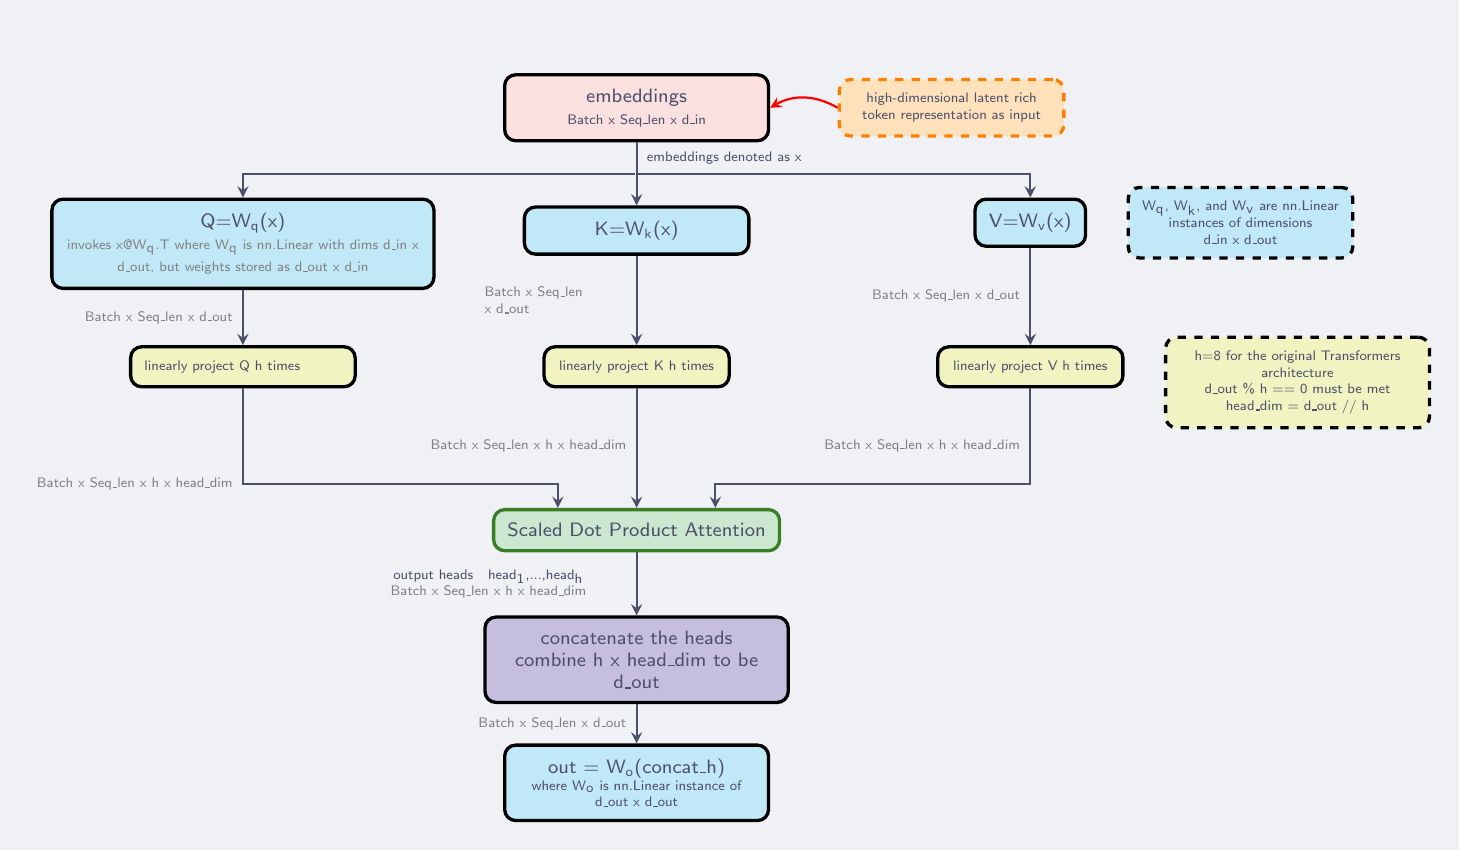
\begin{tikzpicture}[
    BIR/.style={rectangle, draw=black!60, fill=black!5, very thick, minimum size=5mm, minimum height=4em, minimum width=6em},
    RIR/.style={draw=black, very thick, rectangle, rounded corners, inner sep=5pt, inner ysep=5pt}
    ]
    \tikzstyle{every node}=[font=\virgil\scriptsize]
    \node (ref) at (0,0){}; % needs be set as global coordinate
    % node for embeddings
    \node[RIR,fill=sstart] (head) at (4.5, -0.9) {\parbox{3cm}{\centering embeddings\\{\tiny Batch x Seq\_len x d\_in}}};
    % explaining embeddings
    \node [RIR, fill=sorange, draw=orange,dashed] (lrich) at ($(head)+(4, 0)$) {\parbox{2.5cm}{\tiny \centering high-dimensional latent rich token representation as input}};
    \draw [->,thick,red,>=stealth] (lrich.west) to [out=150,in=30] (head.east);
    % three arrows extengin from ebeddings
    \draw[->, thick,>=stealth] (head.south) -- node[name=midh,inner sep=0, outer sep=0]{} node[pos=0.25,right]{{\tiny embeddings denoted as x}} ++ (0, -0.8) node[name=endl1, inner sep=0]{};
    \draw[->, thick,>=stealth] (midh) -- ++ (5,0) -- ++ (0, -0.3) node[name=endl2, inner sep=0]{};
    \draw[->, thick,>=stealth] (midh) -- ++ (-5,0) -- ++ (0, -0.3) node[name=endl3, inner sep=0]{};
    % nodes for matrix multiplication
    \node[RIR,fill=sblue, anchor=north] (q) at (endl3) {
        \parbox{4.5cm}{\centering Q=W\textsubscript{q}(x)\\
        \textcolor{black!50}{\tiny invokes x@W\textsubscript{q}.T where W\textsubscript{q} is nn.Linear 
        with dims d\_in x d\_out, but weights stored as d\_out x d\_in}}};
    \node[RIR,fill=sblue, anchor=north] (k) at (endl1) {
        \parbox{2.5cm}{\centering K=W\textsubscript{k}(x)}};
    \node[RIR,fill=sblue, anchor=north] (v) at (endl2) {V=W\textsubscript{v}(x)};
    % explain expand nodes
    \node [RIR, draw=black,dashed,fill=sblue, anchor=west] at ($(v.east)+(0.5,0)$) {
        \parbox{2.5cm}{\tiny \centering W\textsubscript{q}, W\textsubscript{k}, and W\textsubscript{v} 
        are nn.Linear instances of dimensions \\d\_in x d\_out
        }
    };
    % arrows from Q to Qproj
    \draw[->, thick, >=stealth] (q.south) -- node[left]{\textcolor{black!50}{\tiny Batch x Seq\_len x d\_out}} ++ (0,-0.7) node[name=q1]{};
    
    % nodes for projections of the q, k, and v h times
    \node[RIR, fill=syellow, anchor=north] (qproj) at (q1) {
    \parbox{2.5cm}{\tiny linearly project Q h times}};
    \draw let \p1 = (qproj.north), \p2 = (k.south) in node[RIR, fill=syellow, anchor=north] (kproj) at (\x2, \y1) {
        \parbox{2cm}{\tiny \centering linearly project K h times}
    };
    \draw let \p1 = (qproj.north), \p2 = (v.south) in node[RIR, fill=syellow, anchor=north] (vproj) at (\x2, \y1) {
        \parbox{2cm}{\tiny \centering linearly project V h times}
    };
    % arrows from K, V to K proj, V proj respectively
    \draw[->, thick, >=stealth] (k.south) -- node[left]{\textcolor{black!50}{\tiny \parbox{1.8cm}{Batch x Seq\_len\\ x d\_out}}} (kproj.north) node[name=k1]{};
    \draw[->, thick, >=stealth] (v.south) -- node[left]{\textcolor{black!50}{\tiny Batch x Seq\_len x d\_out}} (vproj.north) node[name=v1]{};
    % explain expand nodes
    \node [RIR, draw=black,dashed,fill=syellow, anchor=west] at ($(vproj.east)+(0.5,-0.2)$) {
        \parbox{3cm}{\tiny \centering h=8 for the original Transformers architecture\\
        d\_out \% h == 0 must be met\\
        head\_dim = d\_out // h}
    };
    % SDPA node
    \node[RIR,fill=sgreen, draw=OliveGreen] (sdpa) at ($(kproj.south)+(0, -1.8)$) {Scaled Dot Product Attention};
    % arrows from projection nodes to SDPA
    \draw[->,thick,>=stealth] (qproj.south) |- node[left]{\textcolor{black!50}{
        \tiny Batch x Seq\_len x h x head\_dim}
    } ($(sdpa.north)+(-1,0.3)$) -- ($(sdpa.north)+(-1,0)$);
    \draw[->,thick,>=stealth] (kproj.south) |- node[pos=0.3,left]{\textcolor{black!50}{
        \tiny Batch x Seq\_len x h x head\_dim}
    } ($(sdpa.north)+(0,0.3)$) -- (sdpa.north);
    \draw[->,thick,>=stealth] (vproj.south) |- node[pos=0.3,left]{\textcolor{black!50}{
        \tiny Batch x Seq\_len x h x head\_dim}
    } ($(sdpa.north)+(1,0.3)$) -- ($(sdpa.north)+(1,0)$);
    % output from SDPA node
    \node [RIR,anchor=north, fill=spurple] (outheads) at ($(sdpa.south)+(0,-0.8)$){
        \parbox{3.5cm}{
            \centering concatenate the heads\\
            combine h x head\_dim to be d\_out}};
    % arrow from SDPA to heads node
    \draw[->,thick,>=stealth] (sdpa.south) -- node[left,pos=0.5]{
        \parbox{3.5cm}{\tiny \centering output heads\quad head\textsubscript{1},...,head\textsubscript{h}\\
        \textcolor{black!50}{Batch x Seq\_len x h x head\_dim}
    }} (outheads.north);
    % Linear matrix multiplication 
    \node[RIR,fill=sblue,anchor=north] (lmm) at ($(outheads.south)+(0,-0.5)$) {
        \parbox{3cm}{\centering
      out = W\textsubscript{o}(concat\_h)\\
      \tiny where W\textsubscript{o} is nn.Linear instance of\\ d\_out x d\_out
    }};
    % arrow from concat to linear mm
    \draw[->,thick, >=stealth](outheads.south) -- node[pos=0.5,left]{\textcolor{black!50}{\tiny Batch x Seq\_len x d\_out}} (lmm.north);
\end{tikzpicture}
\end{minipage}%
\hspace{25pt}
\begin{minipage}[t]{.4\textwidth}
  \raggedright
  \scriptsize 
  $^{11}$ {\it nn.Linear} is an instance initialization of a stack of perceptrons in a single layer in PyTorch, 
  with {\it d\_in} previously known as the abstract dim of the word embedding, and  {\it d\_out} is initialized 
  as {\it d\_in}\\
  \vspace{2em}
  $^{12}$ proving the invocation that initializes Q, K and V matrices
  \begin{lstlisting}[language=python,style=python,basicstyle=\ttfamily\tiny]
import torch
import torch.nn as nn
x = torch.randn(10, 3)
Wq = torch.nn.Linear(3, 40, bias=False)
torch.equal(Wq(x), x.dot(Wq.weight.T))
torch.equal(Wq(x), x@Wq.weight.T) # True
  \end{lstlisting}
  \vspace{2em}
  $^{13}$ the MHA has its core in attention mechanism whose goal is to dynamically decide on 
  which inputs we want to “attend” more than others based on 
  \begin{itemize}[left=0pt,topsep=0pt,itemsep=-1ex,parsep=0ex]
    \item \textbf{\textit{query}} {\tiny $\sim$} a feature vector that describes what we are looking for in the sequence, i.e. what would we maybe want to pay attention to.
    \item \textbf{\textit{keys}} {\tiny $\sim$} for each input element, we have a key which is again a feature vector. This feature vector roughly describes what 
    the element is “offering”, or when it might be important. The keys should be designed such that we can identify the elements we want to pay attention to based on the query.
  \end{itemize}
  $\ldots$
\end{minipage}
\end{figure}
\pagebreak
% PAGE 7
\begin{figure}[!htb]
    \begin{minipage}[t]{0.65\textwidth}
    \raggedright
    \customtext{xtitle}{-1em}{Scaled dot product attention}\\
    The term, first introduced in the {\it Vaswani et al.} paper, involves the following key operations:
    \begin{itemize}[left=0pt,topsep=0pt,itemsep=-1ex,parsep=0ex]
        \item compute the dot product of queries and keys of dimension $d_k$, $QK^T$
        \item scaling by a factor $1/\sqrt{d_k}$ to counteract the effect of extremely small gradients in the 
        softmax computation as will be seen in the next step when $d_k$ becomes very large\sidecite{14}.
        This begets the attention scores.
        \item softmax computation of the normalized result attention scores. The result is the attention weights.
        \item dot product of the attention weights and the values.
      \end{itemize}
      \vspace{1em}
      the infamous equation is therefore\\
      \vspace{-2em}
      \begin{gather*}
          \text{attention}(Q,K,V)=\text{softmax}\left(\frac{QK^T}{\sqrt{d_k}}\right)V
      \end{gather*}
      \begin{figure}[H]
        \centering
        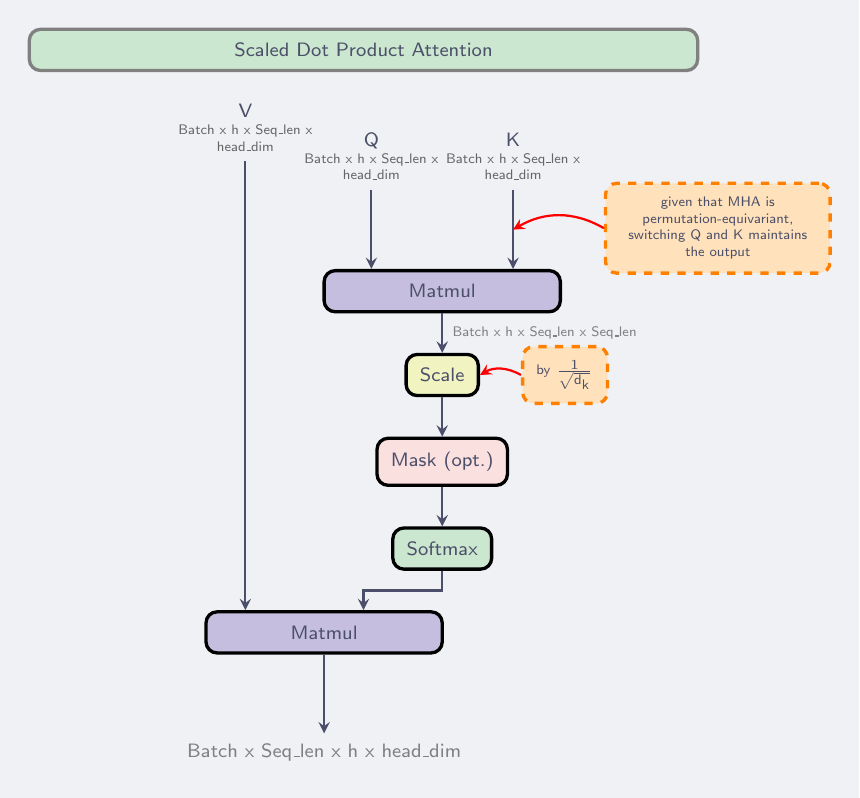
\begin{tikzpicture}[
          RIR/.style={draw=black, very thick, rectangle, rounded corners, inner sep=5pt, inner ysep=5pt}
          ]
          \tikzstyle{every node}=[font=\virgil\scriptsize]
          \node[RIR,fill=sgreen, draw=black!50, minimum width=0.7\textwidth] (sdpa) {Scaled Dot Product Attention};
          \node[RIR, anchor=north,minimum width=3cm,fill=spurple] (matmul) at ($(sdpa.south)+(1,-2.5)$) {Matmul};
          \node[RIR, anchor=north,fill=syellow] (scale) at ($(matmul.south)+(0,-0.5)$) {Scale};
          \node[RIR, anchor=north,fill=sstart] (mask) at ($(scale.south)+(0,-0.5)$) {Mask (opt.)};
          \node[RIR, anchor=north,fill=sgreen] (sm) at ($(mask.south)+(0,-0.5)$) {Softmax};
          \node[RIR, anchor=north,minimum width=3cm,fill=spurple] (matmul2) at ($(sm.south)+(-1.5,-0.5)$) {Matmul};
          % ARROWS
          \draw[<-,thick,>=stealth] ($(matmul.north)+(-0.9,0)$) -- ++ (0, 1) node[above]{\parbox{2cm}{\centering Q\\\tiny \textcolor{black!60}{Batch x h x Seq\_len x head\_dim}}};
          \draw[<-,thick,>=stealth] ($(matmul.north)+(0.9,0)$) -- ++ (0, 1) node[above]{\parbox{2cm}{\centering K\\\tiny \textcolor{black!60}{Batch x h x Seq\_len x head\_dim}}};
          \draw[->,thick,>=stealth] (matmul) -- node[right]{\tiny \textcolor{black!50}{Batch x h x Seq\_len x Seq\_len}} (scale);
          \draw[->,thick,>=stealth] (scale) -- (mask);
          \draw[->,thick,>=stealth] (mask) -- (sm);
          \draw[->,thick,>=stealth] (sm.south) |- ($(matmul2.north)+(0.5,0.25)$) -- ($(matmul2.north)+(0.5,0)$);
          \draw[<-,thick,>=stealth] ($(matmul2.north)+(-1,0)$) -- ++ (0,5.7) node[above]{\parbox{2cm}{\centering V\\\tiny \textcolor{black!60}{Batch x h x Seq\_len x head\_dim}}};
          \draw[->,thick,>=stealth] (matmul2.south) -- ++ (0,-1) node[below]{\textcolor{black!50}{Batch x Seq\_len x h x head\_dim}};
          % explaining 
        \node [RIR, fill=sorange, draw=orange,dashed] (lrich) at ($(matmul)+(3.5,0.8)$) {
            \parbox{2.5cm}{\tiny \centering given that MHA is permutation-equivariant, switching Q and K maintains the output}
            };
        \draw [->,thick,red,>=stealth] (lrich.west) to [out=150,in=30] ($(matmul.north)+(0.9,0.5)$);
        % comment on scale
        \node [RIR, fill=sorange, anchor=west, draw=orange,dashed] (lscale) at ($(scale)+(1,0)$) {
            \tiny \centering by $\frac{1}{\sqrt{\text{d\textsubscript{k}}}}$};
        \draw [->,thick,red,>=stealth] (lscale.west) to [out=150,in=30] (scale.east);
        \end{tikzpicture}
      \end{figure}
      From the diagram above, there's a new block, \bandi{Mask}, that does something called masking. A transformer usually has two phases,
      encoding phase and the decoding phase. From the Transformers architecture diagram, encoder is on the left and the decoder on the right 
      for the two phases.
\end{minipage}%
\hspace{25pt}
\begin{minipage}[t]{.4\textwidth}
  \raggedright
  \scriptsize 
    \fontsize{9}{8}\textcolor{xtitle}{\it from previous $^{13}$...}\\
    \begin{itemize}[left=0pt,topsep=0pt,itemsep=-1ex,parsep=0ex]
        \item \textbf{\textit{values}} {\tiny $\sim$} for each input element, we also have a value vector. This feature vector is the one we want to average over.
        \item \textbf{\textit{score function}} {\tiny $\sim$} to rate which elements we want to pay attention to, we need to specify a score function. The score function 
        takes the query and a key as input, and outputs the score (attention weight) of the query-key pair. It is usually implemented by simple similarity metrics like 
        a dot product, or a small MLP.
    \end{itemize}
    
\includegraphics[width=.1\textwidth]{images/hand-point-up.png}
    \textbf{
                \textit{courtesy of \href{https://uvadlc-notebooks.readthedocs.io/en/latest/tutorial_notebooks/tutorial6/Transformers_and_MHAttention.html}{UvA course notes}}
                }\\
    \vspace{2em}
    $^{14}$ $d_k$ is the size of the last dimension of the keys after linear projection and transpose, to be implemented later.
    It is the head dimension for each attention head.\\ 
    Sanity check states that your key dimension be {\it B x Seq\_len x h x head\_dim}
    before this step where $d_k$ is gotten by {\it k.shape[-1]}
\end{minipage}
\end{figure}
\pagebreak 
% PAGE 8
\begin{figure}[!htb]
    \begin{minipage}[t]{0.65\textwidth}
    \raggedright
    During the decoding phase, at each step of predicting a word\sidecite{15}, the network needs take a look 
    at the words previous to that step, and output a softmax prediction for what it thinks the next word 
    is. Since transformers attend to the entire sequence, before and after, it becomes a trivial task to predict 
    the next word, simply by putting 100\% attention to the word after it.\\
    This of course is cheating, it won't learn anything really. During the inference pipeline, the entire sequence 
    won't be present, hence why we need the masking block, we don't want each word in the decoder to see the words 
    that come after it.\\
    \customtext{xtitle}{1em}{Implementing masking in code}\\
    Let's use the sequence below\\
    {\it Eiffel Tower is in Paris}\\
    and consider the llama 2 tokenizer\sidecite{16}, {\it sentencepiece}, as the final Transformers model built on these progressive learnings  
    while building on the architecture is Llama 2.
\begin{lstlisting}[language=python,style=python,basicstyle=\ttfamily\footnotesize]
import sentencepiece as spm 
sequence = "Eiffel Tower is in Paris"
sp = spm.SentencePieceProcessor("llama-2-7b-tok.model")
tokens = sp.encode_as_ids(sequence)
\end{lstlisting}
Considering V and D used for {\it Llama2 model 7B} variant, let's initialize an embedding instance. 
\begin{lstlisting}[language=python,style=python,basicstyle=\ttfamily\footnotesize]
V,D=32_000,4_096
emb = nn.Embedding(V, D)
emb_tokens = emb(torch.tensor(tokens))
print(emb_tokens.shape)
# torch.Size([7, 4096])
\end{lstlisting}
Our embeddings output being the input to scaled dot product attention, let's compute $QK^T$ then scale
keeping in mind that the batch dimension, multiple heads, and the positional encoding is not incorporated 
for the sake of focusing on masking.
\begin{lstlisting}[language=python,style=python,basicstyle=\ttfamily\footnotesize]
Wq, Wk, Wv = nn.Linear(D,D),nn.Linear(D,D),nn.Linear(D,D)
q, k, v = Wq(emb_tokens), Wk(emb_tokens), Wv(emb_tokens)
scores=q@k.T
scaled_scores=scores/k.shape[-1]**.5
print(scaled_scores.shape) # torch.Size([7, 7])
\end{lstlisting}
% weights=torch.softmax(scaled_scores,dim=-1)
\end{minipage}%
\hspace{25pt}
\begin{minipage}[t]{.4\textwidth}
  \raggedright
  \scriptsize 
  $^{15}$ the model actually predicts a token which, by using a lookup table, is decoded to a word which 
  is what humans understand.\\
  \vspace{2em}
  $^{16}$ the lookup-table {\it tokenizer.model} can be found from the huggingface model card for {\it Llama-2-7b}
  {\tiny \url{https://huggingface.co/meta-llama/Llama-2-7b/tree/main}}
\end{minipage}
\end{figure}
\pagebreak
% PAGE 9
\begin{figure}[!htb]
    \begin{minipage}[t]{0.65\textwidth}
    \raggedright
    
\begin{lstlisting}[language=python,style=python,basicstyle=\ttfamily\tiny]
torch.set_printoptions(precision=5,sci_mode=False,linewidth=500)
print(scaled_scores)
tensor([[-0.10457, -0.23802,  0.08053,  0.33000, -0.10408,  0.55068,  0.68916],
        [-0.35013, -0.04846,  0.65688,  0.18756, -0.81784,  0.10682, -0.74313],
        [-0.26961, -0.70423,  0.94224,  0.16090, -0.20169,  0.15549, -0.28134],
        [-0.32253,  0.56740,  0.08793, -0.53429, -0.19362, -0.22245, -0.38808],
        [ 0.32020,  0.29380,  0.18501, -0.53281,  0.02592, -0.57664,  0.17737],
        [ 0.00706, -0.08485, -0.11895,  0.21021,  0.50643,  0.48187,  0.11625],
        [ 0.38275,  0.45847, -0.34459, -0.12443,  0.35930,  0.65530,  0.03805]], 
        grad_fn=<DivBackward0>)
\end{lstlisting}
Now onto a mask with ones from the first upper off-diagonal onwards. Then, fill them with {\small $-\infty$}
such that the exponential of those values will be zero in the weights. 
\begin{lstlisting}[language=python,style=python,basicstyle=\ttfamily\footnotesize]
mask = torch.triu(torch.ones_like(scaled_scores), diagonal=1)
scaled_scores_masked = scaled_scores.masked_fill_(mask.bool(), -torch.inf)
weights = torch.softmax(scaled_scores_masked, dim=-1)
\end{lstlisting}
Now, for the weights, pre-matrix multiply with {\small V} for the result of Scaled Dot Product Attention
\begin{lstlisting}[language=python,style=python,basicstyle=\ttfamily\footnotesize]
out = weights @ v 
print(out.shape) # torch.Size([7, 4096])
\end{lstlisting}
Nice! Now onto {\it Add \& Norm} layer, which from the paper, is a Layer normalization that computes\\
\vspace{-1.5em}
$$\text{LayerNorm}(x  + \text{Multihead(}x, x, x))$$
where $x$ is basically the same sequence (as an embedding) input to the $Q, K \& V$. This layer hence
is a residual connection necessary for enabling smooth gradient flow through the model and retaining 
information from the original sequence prior to the multi-head attention. This is simply implemented as 
\begin{lstlisting}[language=python,style=python,basicstyle=\ttfamily\footnotesize]
out_attn = multiheadAttn(x)
out = x + out_attn
norm_out = norm(out)
\end{lstlisting}
\customtext{xtitle}{0em}{What about the Feed Forward NN layer}\\
Always forming a crucial layer in most models, the FFN, in this case, 
maps context rich vectors onto a higher dimension\sidecite{17} which increases learning 
so it can model more complex relationships and also adds an activation 
function to introduce non-linear, even better relations.
\end{minipage}%
\hspace{25pt}
\begin{minipage}[t]{.4\textwidth}
  \raggedright
  \centering
  \scriptsize 
  $^{17}$ \textcolor{xtitle}{\it Feed Forward NN layer for Transformer model}\\
  \vspace{1em}
    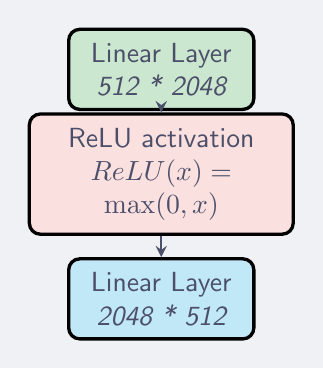
\begin{tikzpicture}[
    BIR/.style={rectangle, draw=black!60, fill=black!5, very thick, minimum size=5mm, minimum height=4em, minimum width=6em},
    RIR/.style={draw=black, very thick, rectangle, rounded corners, inner sep=5pt, inner ysep=5pt}
    ]
        \node[RIR, fill=sgreen] (L1) {\parbox{2cm}{\centering Linear Layer\\{\it 512 * 2048}}};
        \node[RIR, fill=sstart] (L2) at  ($(L1.south)+(0,-0.8)$) {\parbox{3cm}{\centering ReLU activation\\{$ReLU(x)=\max(0,x)$}}};
        \draw[thick,->,>=stealth] (L1.south) -- (L2.north);
        \node[RIR, fill=sblue] (L3) at  ($(L2.south)+(0,-0.8)$) {\parbox{2cm}{\centering Linear Layer\\{\it 2048 * 512}}};
        \draw[thick,->,>=stealth] (L2.south) -- (L3.north);
    \end{tikzpicture}\\
  \vspace{1em}
  \textcolor{xtitle}{\it Feed Forward NN layer for GPT-2}\\
  \vspace{0.5em}
    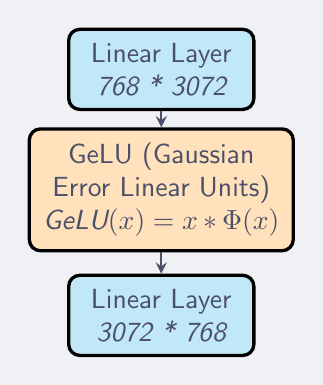
\begin{tikzpicture}[
    BIR/.style={rectangle, draw=black!60, fill=black!5, very thick, minimum size=5mm, minimum height=4em, minimum width=6em},
    RIR/.style={draw=black, very thick, rectangle, rounded corners, inner sep=5pt, inner ysep=5pt}
    ]
        \node[RIR, fill=sblue] (L1) {\parbox{2cm}{\centering Linear Layer\\{\it 768 * 3072}}};
        \node[RIR, fill=sorange] (L2) at  ($(L1.south)+(0,-1)$) {\parbox{3cm}{\centering GeLU (Gaussian Error Linear Units)\\{$\text{\it GeLU}(x)=x*\Phi(x)$}}};
        \draw[thick,->,>=stealth] (L1.south) -- (L2.north);
        \node[RIR, fill=sblue] (L3) at  ($(L2.south)+(0,-0.8)$) {\parbox{2cm}{\centering Linear Layer\\{\it 3072 * 768}}};
        \draw[thick,->,>=stealth] (L2.south) -- (L3.north);
    \end{tikzpicture}
    \vspace{1em}\\
    \textcolor{xtitle}{\it Feed Forward NN layer for Llama-2-7b}\\
    \vspace{0.5em}
    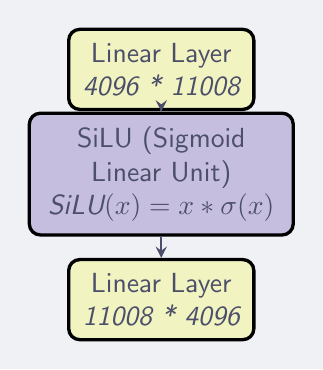
\begin{tikzpicture}[
    BIR/.style={rectangle, draw=black!60, fill=black!5, very thick, minimum size=5mm, minimum height=4em, minimum width=6em},
    RIR/.style={draw=black, very thick, rectangle, rounded corners, inner sep=5pt, inner ysep=5pt}
    ]
        \node[RIR, fill=syellow] (L1) {\parbox{2cm}{\centering Linear Layer\\{\it 4096 * 11008}}};
        \node[RIR, fill=spurple] (L2) at  ($(L1.south)+(0,-0.8)$) {\parbox{3cm}{\centering SiLU (Sigmoid Linear Unit)\\{$\text{\it SiLU}(x)=x*\sigma(x)$}}};
        \draw[thick,->,>=stealth] (L1.south) -- (L2.north);
        \node[RIR, fill=syellow] (L3) at  ($(L2.south)+(0,-0.8)$) {\parbox{2cm}{\centering Linear Layer\\{\it 11008 * 4096}}};
        \draw[thick,->,>=stealth] (L2.south) -- (L3.north);
    \end{tikzpicture}
\end{minipage}
\end{figure}
\pagebreak
% PAGE 10
\begin{figure}[!htb]
    \begin{minipage}[t]{0.65\textwidth}
    \raggedright
    \customtext{xtitle}{0em}{Building Llama-2 from the SDPA outwards...}\\
Gladly having gone through the layers in the Transformer model, it is of essence 
to build the Llama-2 model graph and load the weights for the 7B variant. 
It is a decoder-only architecture, as is most State of The Art common LLMs.
Why is that?\\
Well, decoder-only architectures worked very well for next token prediction and translation tasks, 
and were easier to train.
% \begin{lstlisting}[language=python,style=python,basicstyle=\ttfamily\footnotesize]
% mask = torch.triu(torch.ones_like(scaled_scores), diagonal=1)
% scaled_scores_masked = scaled_scores.masked_fill_(mask.bool(), -torch.inf)
% weights = torch.softmax(scaled_scores_masked, dim=-1)
% \end{lstlisting}
even better relations.
\end{minipage}%
\hspace{25pt}
\begin{minipage}[t]{.4\textwidth}
  \raggedright
  \scriptsize 
\end{minipage}
\end{figure}
\end{document}
